\chapter{Results}
\section{Virtual Prototyping of Cell Signals}

During the course of this thesis, numerical simulations for the microchannel have been carried out. On the one side, a simulation about the shape of a \gls{gmr}-sensor signal of cells was performed, where the magnetic momentum was conveyed through \glspl{mnp} bound to their surface. On the other side, cell aggregates have been looked at in the same manner with different angles respective to the sensor. Both simulations were then correlated to a reference dipole, with the equivalent magnetic momentum distributed in the center of mass.\\
Additionally, the flow and shear field inside the channel was simulated numerically for the channel cross section as well as for a particle near the walls. A force equilibrium simulation was also established in a basic manner. \\
Every simulation was captured in a MATLAB class ``MRCyte'', which contains material parameters and constants for all simulations above.
\subsection{Numerical investigation of immunomagnetic label density and size on quantitative magnetoresistive sensing of single cells and cell aggregates}
In order to mimic a immunomagnetically labeled cell flowing over the sensor half bridge, the planar integral of the respective \acrfull{B} was solved analytically. Here, $\mathbf{r}_i$ specifies the distance vector of a single \gls{mnp} from the sensor plane. The magnetic flux density was converted by the \gls{gmr} to a resistive change $\mathbf{R}_{sig}$ by scaling it with the \gls{gmr}-sensitivity $S$ and subsequently into a signal voltage $\mathbf{V}_{sig}$ inside the bridge branch.(\cref{eq:magneticFluxIntegral,eq:GMR-signal,eq:voltage-signal})\\
In the numerical approach, \glspl{mnp} were randomly sampled on a sphere surface with an equivalent diameter of \SI{4}{\micro\meter} or \SI{8}{\micro\meter}. Then, the signal was computed for every \gls{mnp} during every timestep. Additionally, the \gls{mnp} distribution was rotated in every iteration to resemble a rolling motion. The computed signals were then cross-correlated to the signal of a reference flux density $\mathbf{B}_{ref}$ caused by a point-like magnetic moment located in the geometric center of the same sphere.
\begin{align}
	\mathbf{B}(t) &= \sum_{i=1}^{N} \frac{1}{A_{\mathrm{Sensor}}} \int_{-\frac{l}{2}}^{\frac{l}{2}} \int_{-\frac{w}{2}}^{\frac{w}{2}} \frac{\mu_{o}}{4 \pi}\left(\frac{3 \mathbf{r}_{i}(t)\left(\mathbf{r}_{i}(t) * \mathbf{m}_{i}\right)}{\left|\mathbf{r}_{i}(t)\right|^{5}}-\frac{\mathbf{m}_{i}}{\left|\mathbf{r}_{i}(t)\right|^{3}}\right) dx dy \label{eq:magneticFluxIntegral} \\
	\mathbf{R}_{sig}(t) &= - \mathbf{B}(t) * \frac{S}{100} * R + R \label{eq:GMR-signal}\\
	\mathbf{V}_{sig}(t) &= \frac{\mathbf{R}_{sig}(t)}{R + \mathbf{R}_{sig}(t)}*V_p - \frac{V_p}{2} \label{eq:voltage-signal}
\end{align}
By its formula, cross-correlation $R_{x y}(\tau)$ yields a displacement dependent signal through its convolution of the complex conjugated reference signal $\mathrm{V}_{ref}^{*}(t)$ with the sample signal $\mathbf{V}_{sig}(t+\tau)$.(\cref{eq:xcorr}) Therefor, only the maximal correlation of this function was considered in further analyses.
\begin{equation}
	\mathrm{max}\{R_{x y}(\tau)\}=\mathrm{max}\left\{\int_{-\infty}^{\infty} \mathrm{V}_{ref}^{*}(t) \mathbf{V}_{sig}(t+\tau) dt \right\} \label{eq:xcorr}
\end{equation}

\begin{figure}
	\centering
	\begin{minipage}[t]{.24\linewidth}
		\subfloat{
			\subfigimg[height=323pt]{a}{Ressources/Simulation/GMR}			
			\phantomsubcaption
			\label{fig:sim:intro:gmr}
		}
	\end{minipage}%
	\hfill
	\begin{minipage}[b]{.7\linewidth}
		\addtocounter{subfigure}{-1}
		\subfloat{
			\subfigimg[width=\linewidth]{b}{Ressources/Simulation/ParticleCoverage}
			\phantomsubcaption
			\label{fig:sim:intro:coverage}
		} 
		\\
		\vspace{\baselineskip}	
		\addtocounter{subfigure}{-1}
		\subfloat{
			\subfigimg[width=\linewidth]{c}{Ressources/Simulation/ParticleAngle}			
			\phantomsubcaption
			\label{fig:sim:intro:angle}
		}
	\end{minipage}%	
	\capption{Particle Coverage Simulation}{(\textbf{a}) Dimensions of the \gls{gmr} Wheatstone bridge sensor: Distance d between both variable bridges (green), width w of a \gls{gmr}-sensor, length L of a sensor. (\textbf{b}) Scheme of single cell simulation: The ideal magnetic dipole in the geometric center of a sphere (\blueCircle) causes a signal deviation from the real cell signal with magnetic moment distributed on the cell surface. (\orangeCircle) (\textbf{c}) Signal shapes of different angles of two-particle aggregates lead to differing signal shapes. }
	\label{fig:sim:intro}	
\end{figure}
\todo{Signal Similarity For Cells With Varying Bead Coverages,Cross-Correlation between single dipole with sum magentic moment and surface covered with randomly distributed magnetic particles, simulation of cell rolling velocity and forces}


\clearpage
\subsection{Single Cell Signal}
Aim of these simulations is to find a measure of how magnetic labeling of a cell affects signal shape and its subsequent analysis. A single cell with a surface coverage of \SIrange{5}{99}{\percent} of a densely packed sphere was loaded randomly with \glspl{mnp} at different sizes. Then, the previously explained rolling motion over the sensor bridge was simulated with the parameters specified in \cref{tab:params:mag_sim}. After correlation of the resulting signal voltage to the reference dipole signal (\cref{fig:sim:intro:coverage}, \blueCircle) with three randomly \gls{mnp} distributions, the dependency on the coverage was evaluated. As shown in the schematic \cref{fig:sim:intro:coverage}, an increase in signal peak amplitude but also in \gls{fwhm} at growing coverage was expected . 

\begin{table}
	\centering
\begin{tabularx}{\linewidth}{cccc}
	\toprule[1pt]
	\rule[-1ex]{0pt}{2.5ex} Parameter & Unit & Value & Explanation \\	
	\midrule
	\rule[-1ex]{0pt}{2.5ex} w & \si{\meter} & \num{2.0e-6} & GMR width \\
	\rule[-1ex]{0pt}{2.5ex} l & \si{\meter} & \num{30.0e-6} & GMR length \\
	\rule[-1ex]{0pt}{2.5ex} d & \si{\meter} & \num{14.0e-6} & Distance between two sensors \\
	\rule[-1ex]{0pt}{2.5ex} $R$ & $\mathrm{\Omega}$ & 250 & GMR Resistance\\
	\rule[-1ex]{0pt}{2.5ex} $V_p$ & \si{\milli\volt} & 100 & Supply voltage\\
	\rule[-1ex]{0pt}{2.5ex} t$_{free\ layer}$ & \si{\meter} & \num{7.0e-9} & Thickness of free layer\\
	\rule[-1ex]{0pt}{2.5ex} $\mathbf{M}$ & \si{\ampere\per\meter} & \num{2.0e4} & Volume Magnetization\\
	\rule[-1ex]{0pt}{2.5ex} $V_{noise,rms}$ & \si{\volt} & \num{2.5e-6} & Artifical noise\\
	\rule[-1ex]{0pt}{2.5ex} Sim. Space & \si{\meter} & [\num{-25e-6},\num{25e-6}] & Interval around sensor center \\	
	\bottomrule[1.2pt]
\end{tabularx}
\capption{Magnetic Simulation Parameters}{Constants used inside the framework for the simulation of the magnetic field inside the \gls{gmr} Wheatstone half bridge. The volume magnetization was adapted according to the simulated particle size.}
\label{tab:params:mag_sim}
\end{table}

The expected behavior matches the data analysis (\cref{fig:sim:coverage}). Each two analyzed sphere diameters \SIlist{4;8}{\micro\meter} with \gls{mnp} sizes ranging from \SI{20}{\nano\meter} to \SI{2}{\micro\meter}, show a great \gls{sem} at low coverage. This very probably is subjected to the momenta of single particles which play a greater individual role and hence influence the signal shape significantly because the overall dipole momentum in the sensor loses homogeneity. \\
Another observable effect is related to the \gls{mnp} size. Absolute correlation differs from \SI{20}{\nano\meter} to the ten and hundered fold diameter significantly. This can be related to the magnetic momentum per \gls{mnp} as it is dependent on the volume - thus $r^3$. However, for bigger magnetic particles this does not hold true because the composition changes from pure magnetite to a polymer shell with embedded oxide core at around \SI{150}{\nano\meter}. Nevertheless, larger particles possess also greater magnetic momentum which brings also the aforementioned influence of single \glspl{mnp} into consideration for that effect. \\ 
Also, the densely packed sphere surface can evidently carry more smaller than larger \glspl{mnp}. This ranges from \num{641600} \gls{mnp} at \SI{20}{\nano\meter} to \num{81} at \SI{2}{\micro\meter} for a sphere radius of \SI{4}{\micro\meter} and limits the maximum achievable momentum. \\
In reality, a maximum immunomagnetic label density depends not on the densely packed sphere but rather on the present antigens, and association or dissociation constants. Therefore, a complete saturation coverage is not achievable under physiological conditions. This leads to the fact that any possible momentum by deposition of \SIlist{20;50}{\nano\meter} on a cell surface cannot be resolved from noise by this sensing setup.

\begin{figure}
	\centering
	\subfloat{	
		\subfigimg[height=145pt]{a}{Ressources/Simulation/Small2um}	
		\phantomsubcaption
		\label{fig:sim:coverage:small2um}
	} \hfill
	\addtocounter{subfigure}{-1}
	\subfloat{
		\subfigimg[height=145pt]{b}{Ressources/Simulation/Big2um}
		\phantomsubcaption
		\label{fig:sim:coverage:big2um}	
	} \\
	\vspace{\baselineskip}	
	\addtocounter{subfigure}{-1}
	\subfloat{	
		\subfigimg[height=145pt]{c}{Ressources/Simulation/Small4um}	
		\phantomsubcaption
		\label{fig:sim:coverage:small4um}
	}\hfill
	\addtocounter{subfigure}{-1}
	\subfloat{
		\subfigimg[height=145pt]{d}{Ressources/Simulation/Big4um}
		\phantomsubcaption
		\label{fig:sim:coverage:big4um}
	}
\capption{Coverage Dependent Signal Correlation}{\gls{mnp} coverage of a sphere with \SI{4}{\micro\meter} (\textbf{a}, \textbf{b}) and \SI{8}{\micro\meter}  diameter  (\textbf{c}, \textbf{d}) covered by magnetic particles ranging from \SIrange{20}{2000}{\nano\meter}. A cross-correlation increase which is inversely proportional to the \gls{mnp} size can be observed.}
\label{fig:sim:coverage}
\end{figure}


Also, it can be seen that the correlation approaches a maximum obtainable value for every \gls{mnp} size. Referenced for both simulated sphere diameters in (\cref{fig:sim:CorrDiff:abs}), a inverse proportionality between correlation and \gls{mnp} diameter is visible. The trend in respective maxima can be related to differences the magnetic momentum amplitude and coverage inhomogeneity. \\ 
Inter-sphere compared, maximum correlation shows also a significant decrease in for higher \gls{mnp} sizes as the particle diameter itself increases. The relative error between both sizes - as computed in \cref{eq:sim:relCorrDiff} -  is depicted in \cref{fig:sim:CorrDiff:rel}. Assuming a dependency on the available particle surface and subsequently the fraction which can be occupied by \glspl{mnp}, a quadratic fit seems appropriate.(\cref{eq:sim:quadFit}) The fit could indicate that a reference dipole cannot be discriminated from a cell at small \gls{mnp} diameters while the correlation error becomes nearly constant at great \glspl{mnp}.

\begin{align}
	\text{Relative\ Correlation\ Difference} &= 1- \frac{\max\{\text{Cross-Correlation}(d_{\SI{4}{\micro\meter}})\}}{\max\{\text{Cross-Correlation}(d_{\SI{8}{\micro\meter}})\}} \label{eq:sim:relCorrDiff}\\
	\text{Relative\ Correlation\ Difference} &= \num{-0,38532} \, {d_{MNP}}^2 + \num{3,34574} \, d_{MNP} - \num{8,49629} \label{eq:sim:quadFit}
\end{align}



\begin{figure}
		\centering
	\subfloat{
		\subfigimg[height=150pt]{a}{Ressources/Simulation/CrossCorr-Maximal}
		\phantomsubcaption
		\label{fig:sim:CorrDiff:abs}	
	} \hfill
	\addtocounter{subfigure}{-1}
	\subfloat{
		\subfigimg[height=150pt]{b}{Ressources/Simulation/CrossCorr-Error}	
		\phantomsubcaption
		\label{fig:sim:CorrDiff:rel}
	}
\capption{Maximal Cross-Correlation Differences}{(\textbf{a}) Mean coverage at \SI{99}{\percent} for \SI{4}{\micro\meter}  and \SI{8} {\micro\meter} spheres. A negative dependency on the \gls{mnp} size can be explained by the ratio of magnetic momentum per unit surface and its homogeneous distribution across the whole surface.\\ (\textbf{b}) Relative correlation error between \SI{4}{\micro\meter}  and \SI{8} {\micro\meter} spheres with a quadratic fit. The quadratic behavior could be related to the relative surface area which can occupied by magnetic momentum. (Red. Chi-square = \num{0,02821})}
\label{fig:sim:CorrDiff}
\end{figure}

\subsection{Cell Aggregates}
In another simulation, two \SI{200}{\nano\meter}-\gls{mnp}-covered spheres were attached to each other in differing angles and simulated flowing over the sensor. Signal similarity to a magnetic dipole in the center of a single reference sphere was computed by cross-correlation. As can be observed in \cref{fig:sim:aggregates}, correlation is identical to a single sphere at low coverages when the magnetic momentum is high enough to form a uniform magnetic field. At occupancies greater than \SI{50}{\percent}, the two attached cells have to be considered as individual dipoles in superposition and thus show a signal that carries small peaks in the center. This is shown schematically in \cref{fig:sim:intro:angle}. In term, this causes a high signal deviation from the reference and thus a low degree of correlation.
\begin{figure}
	\centering
	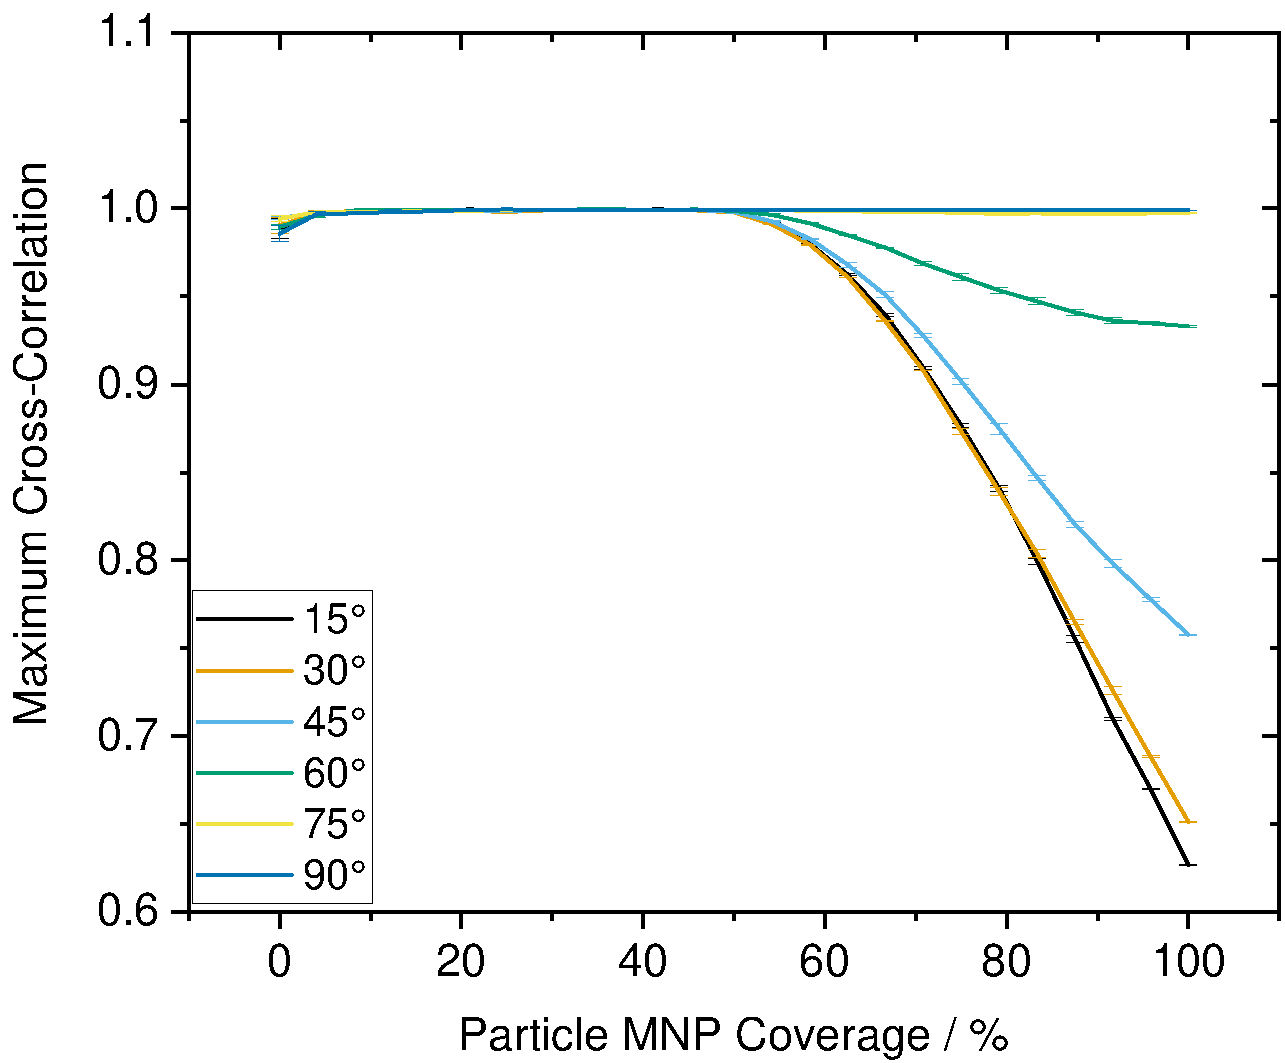
\includegraphics[width=.7\linewidth]{Ressources/Simulation/Aggregates}	
	\capption{Signal Correlation between Two-Cell Aggregates At Shifting Angles}{Two-Sphere aggregates are covered with \SI{200}{\nano\meter} \glspl{mnp} and simulated flowing over the sensor at differing respective angles. The \gls{sem} indicates a difference in cross-correlation of three truly random \gls{mnp} distributions. For low yaw angles and high coverages, the aggregate's signal reflects rather two single dipoles in superposition than one quite homogeneous dipole. This causes a high signal deviation from the reference and thus a low degree of correlation.}
	\label{fig:sim:aggregates}
\end{figure}

\clearpage
\section{Reference Bead Surface Functionalization}
After simulation of the coverages, biotin was titrated on \SI{8}{\micro\meter} reference beads with two different surface terminations in order to selectively bind \glspl{mnp} with the counter-agent streptavidin to the surface. First, \gls{amine}-microbeads were modified by sulfo-NHS-biotin. Second, \gls{carboxyl}-beads were coated by amine-PEG$_2$-biotin via EDC-NHS-activation. On the same beads Anti-IgG1-PE antibodies were titrated after the same coupling chemistry.\\
Subsequently, biotin-coated beads were analyzed in the flow cytometer in the by staining with Atto-488 (Ex: \SI{500}{\nano\meter}, Em: \SI{520}{\nano\meter}) coupled streptavidin. The antibody was already industrially modified with \gls{pe} and measured at \SI{488}{\nano\meter} excitation and \SI{585}{\nano\meter}  emission wavelength. The gating was standardized by the strategy in \cref{sec:meth:beadCharact}, \cref{fig:gatingstrategy-layout}. Subsequently, the \gls{mfi} was computed and fitted with a Hill-function.(\cref{eq:hill})
\begin{table}[!h]

\subfloat{
	\begin{tabularx}{.60\linewidth}[t]{cccc}
		\toprule[1.2pt]
		Param. & Hill \ref{fig:biotinyl:titration:nh2} & Hill \ref{fig:biotinyl:titration:cooh} & Hill \ref{fig:biotinyl:titration:igg} \\
		\midrule
		$V_{max}$ &   \num{173.077} & \num{171,02602} & \num{713.83643}  \\
		$k$ & \num{0.0572831}  & \num{0,04201}  & \num{182.83011} \\
		$n$ &  \num{1.63554} & \num{0,9133} &  \num{0.72458}\\
		Red. $\chi^2$ & \num{275.19597}  & \num{4,07387}  & \num{0.91011}  \\
		\bottomrule
	\end{tabularx}
\phantomsubcaption
\label{tab:biotinyl:fitParams:beads}
} \hfill
\subfloat{
	\begin{tabularx}{.33\linewidth}[t]{cc}
		\toprule[1.2pt]
		Param. & Exp. \ref{fig:biotinyl:titration:stability} \\
		\midrule
		$A$ &   \num{0.91263} \\
		$\tau_{decay}$ & \num{1.42557}  \\
		$y_0$ & \num{0.12369}  \\
		Red. $\chi^2$  & \num{0.00542 } \\
		\bottomrule	\end{tabularx}
	\phantomsubcaption
	\label{tab:biotinyl:fitParams:stability}
}
\capption{Fit Parameters of Biotinylation}{(\textbf{a})}
\label{tab:biotinyl:fitParams}
\end{table}
\begin{align}
	y &= V_{max} \ \frac{x^n}{k^n + x^n} \label{eq:hill} \\
	y &= y_0 + A \exp^{-\frac{x}{\tau_{decay}}}  \label{eq:expDecay}
\end{align}

\subsection{Amine-Surface Biotinylation}
Streptavidin-Atto488 reference calibration
Anti-Biotin-PE working?
BNF-Dextran-Streptavidin unspecific binding?



\begin{figure}
	\centering
	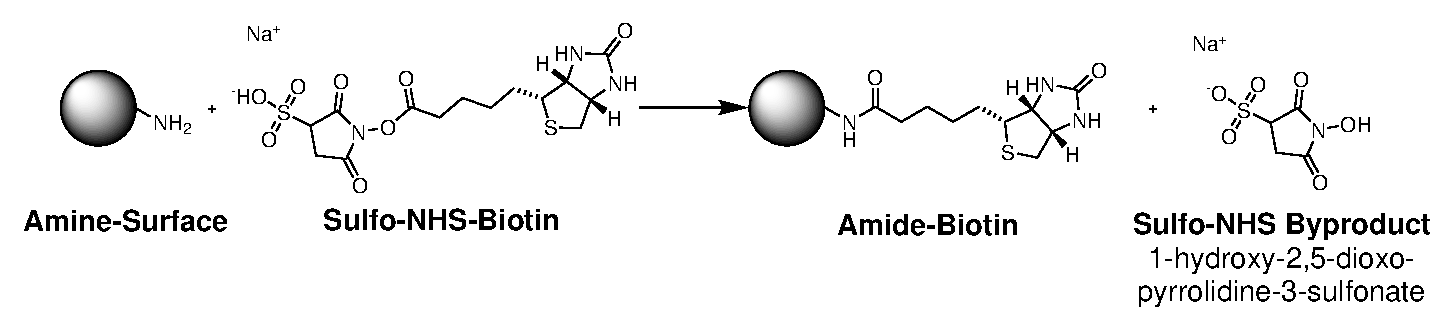
\includegraphics[width=\linewidth]{./Ressources/Chemistry/Sulfo-NHS.eps}
	\capption{Amine Bead Modification with Sulfo-NHS-Biotin}{An amine terminated bead is incubated with sulfo-NHS-Biotin to cover its surface by amide-Biotin. As byproduct the sulfo-NHS-ester 1-hydroxy-2,5-dioxopyrrolidine-3-sulfonate splits off. }
	\label{fig:Chem:NH2-NHS}
\end{figure}


\begin{figure}
	\centering
	\subfloat{
		\subfigimg[height=90pt]{a}{./Ressources/Biotinyl/mag-nh2}	
				\phantomsubcaption
		\label{fig:biotinyl:titration:nh2}
	} \hfill
	\addtocounter{subfigure}{-1}
	\subfloat{
		\subfigimg[height=90pt]{b}{./Ressources/Biotinyl/cooh}	
		\phantomsubcaption
		\label{fig:biotinyl:titration:cooh}
	}\hfill
	\addtocounter{subfigure}{-1}
	\subfloat{
		\subfigimg[height=90pt]{c}{./Ressources/Biotinyl/IgG-cooh}	
		\phantomsubcaption
		\label{fig:biotinyl:titration:igg}
	} \\
	\addtocounter{subfigure}{-1}
	\vspace{\baselineskip}
	\subfloat{
	\subfigimg[height=150pt]{c}{./Ressources/Biotinyl/stability}
	\phantomsubcaption
	\label{fig:biotinyl:titration:stability}	
	}

	\capption{Titration of Biofunctional Molecules on \SI{8}{\micro\meter} Particles}{ (\textbf{a}) NHS-Biotin, MFI, CV,=  n =  (\textbf{b}) Amin-PEG$_2$-Biotin MFI, CV, outlier neglected	(\textbf{c}) MFI, CV, (\textbf{d}) MFI, SEM, }
	\label{fig:biotinyl:titration}
\end{figure}



%\begin{figure}
%	\centering
%	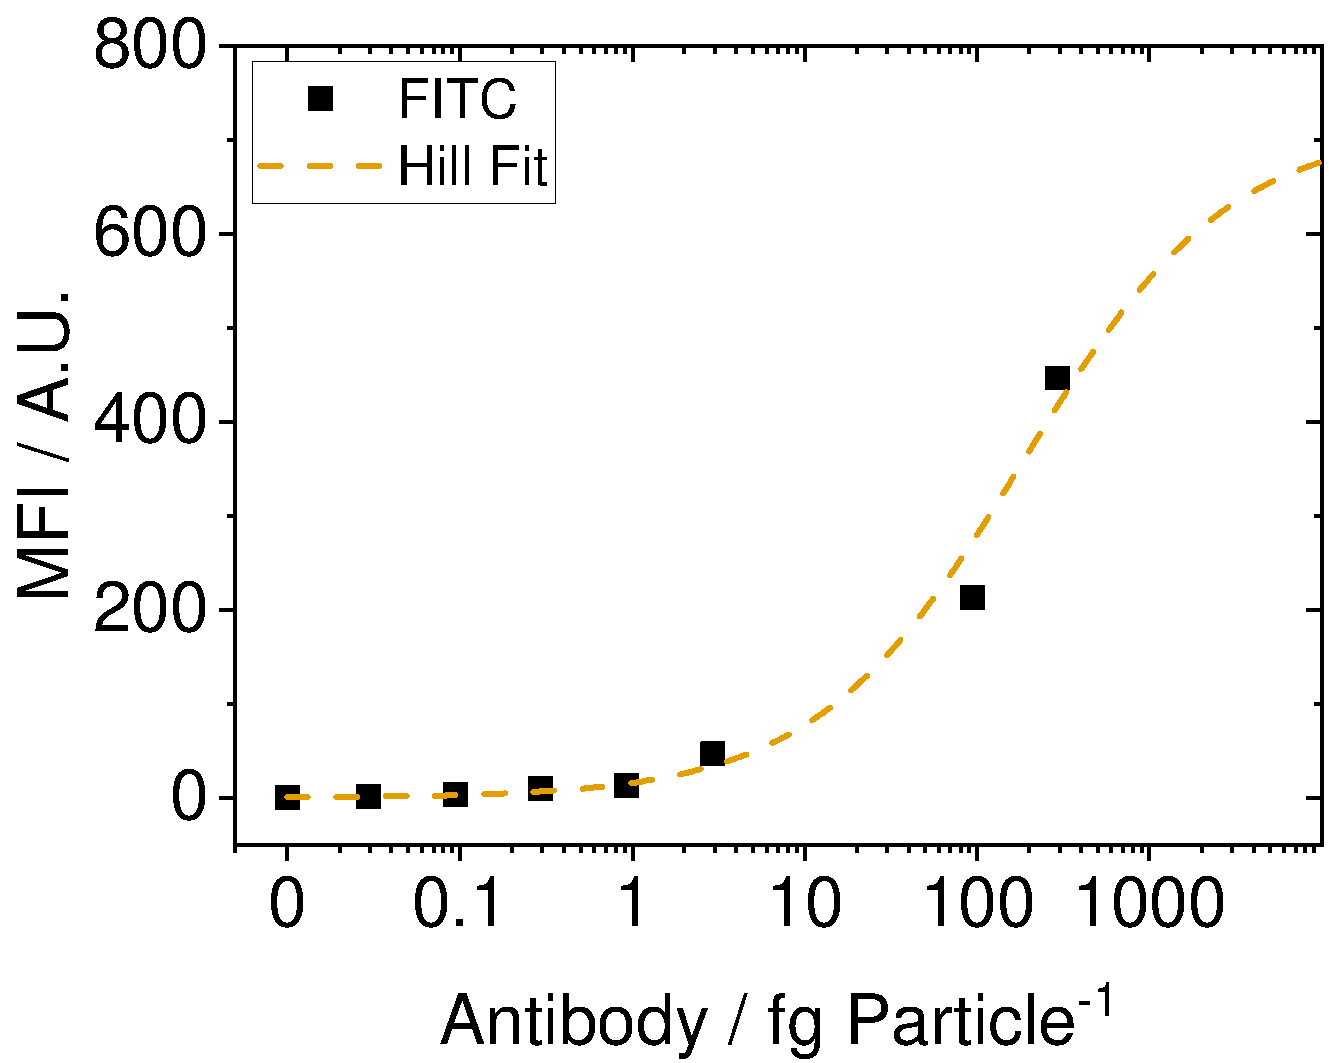
\includegraphics[width=.7\linewidth]{./Ressources/Biotinyl/IgG-cooh}
%	\capption{Titration of Anti-IgG1 on \SI{8}{\micro\meter} Particles}{MFI, CV, reduced chi square = 
%		0.91011, Hill Fit $y=Vmax*x^n/(k^n+x^n)$, Vmax = 713.83643, k = 182.83011	, n = 0.72458 }
%	\label{fig:biotinyl:IgG-cooh}
%\end{figure}

%\begin{figure}
%	\centering
%	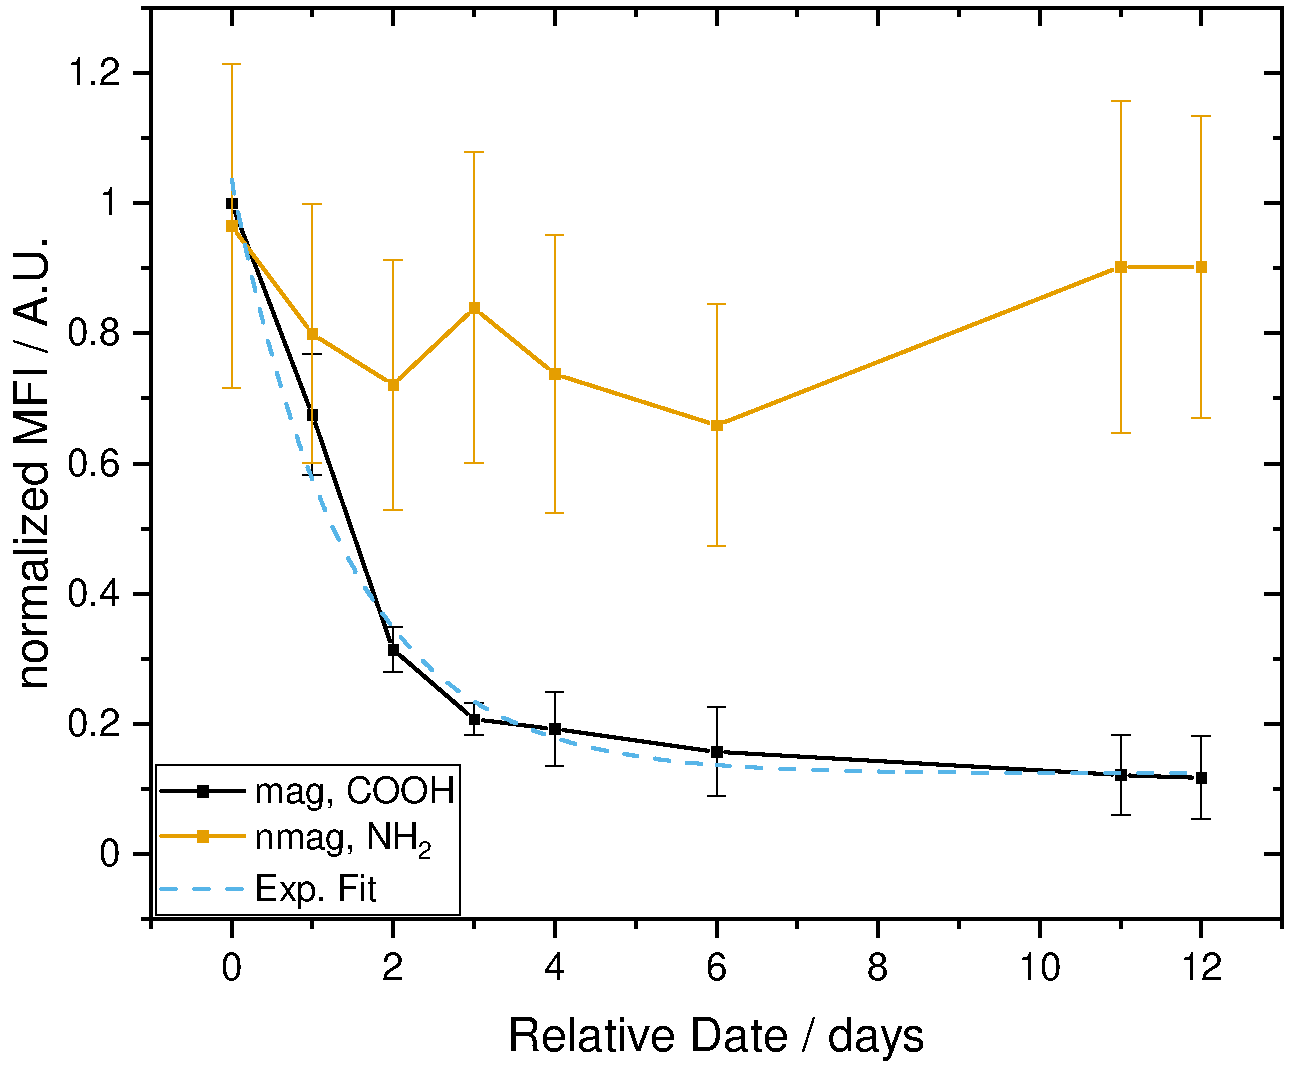
\includegraphics[width=\.7\linewidth]{./Ressources/Biotinyl/stability}
%	\capption{Titration of Anti-IgG1 on \SI{8}{\micro\meter} Particles}{MFI, SEM, reduced chi square = 
%		0.00542, Hill Fit $y=Vmax*x^n/(k^n+x^n)$, Vmax = 713.83643, k = 182.83011	, n = 0.72458 }
%	\label{fig:biotinyl:stability}
%\end{figure}


\section{Concentration Measurements in MRCyte}
Explain v-c
\begin{figure}
	\centering
	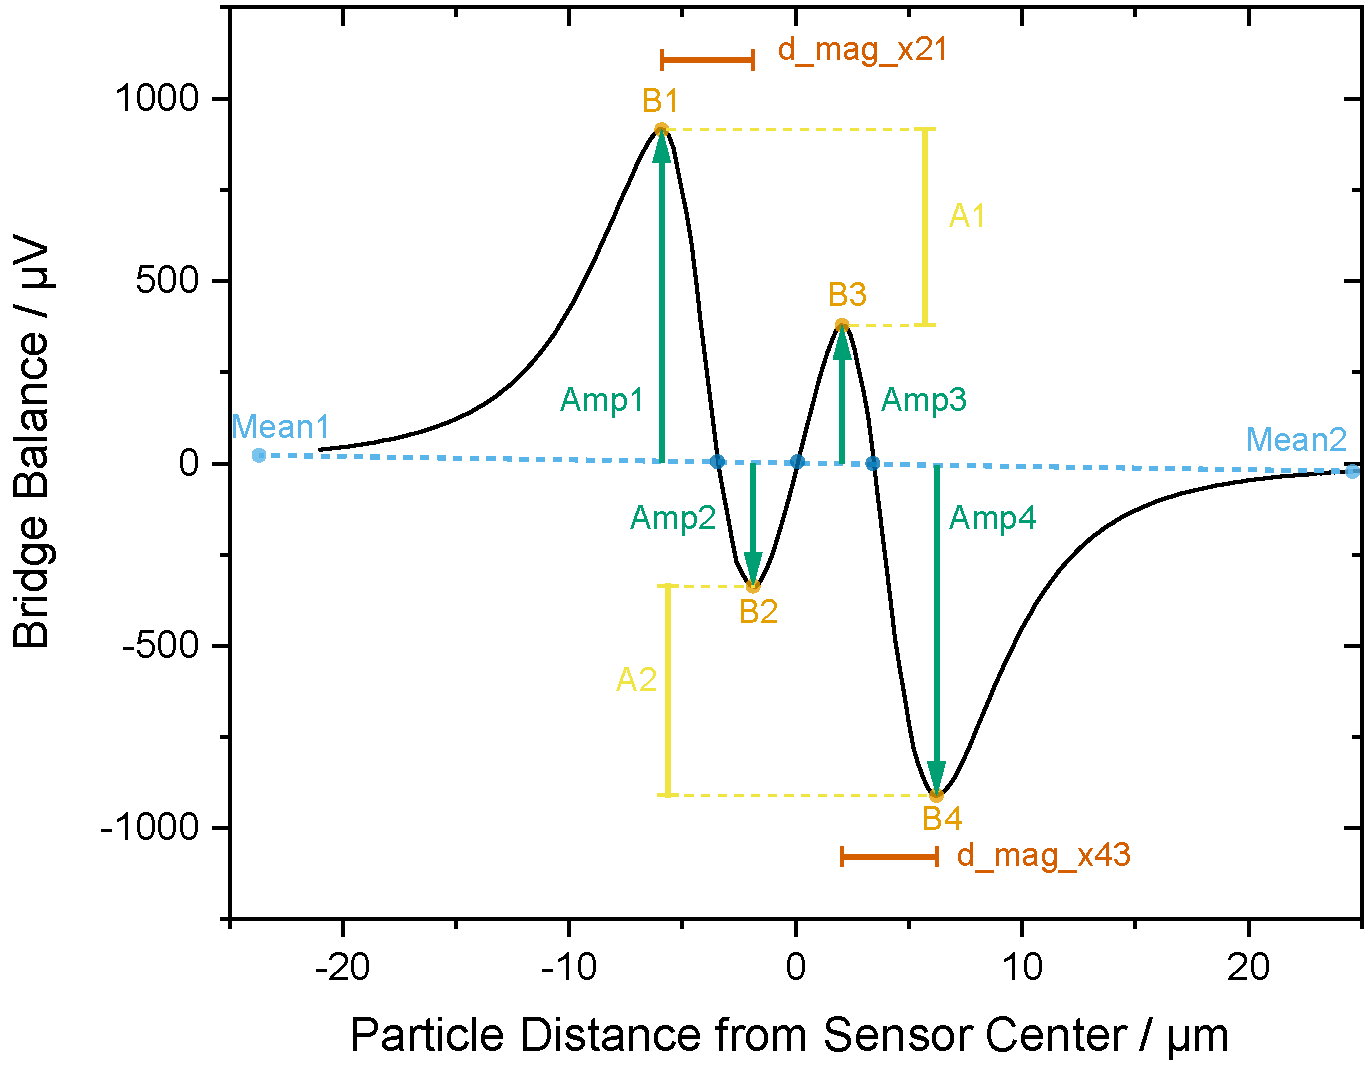
\includegraphics[width=.7\linewidth]{Ressources/Simulation/ExampleSignal}
	\capption{Example Signal of Magnetic Measurement}{explain all}
	\label{fig:conc:example}
\end{figure}

\begin{figure}
	\centering
	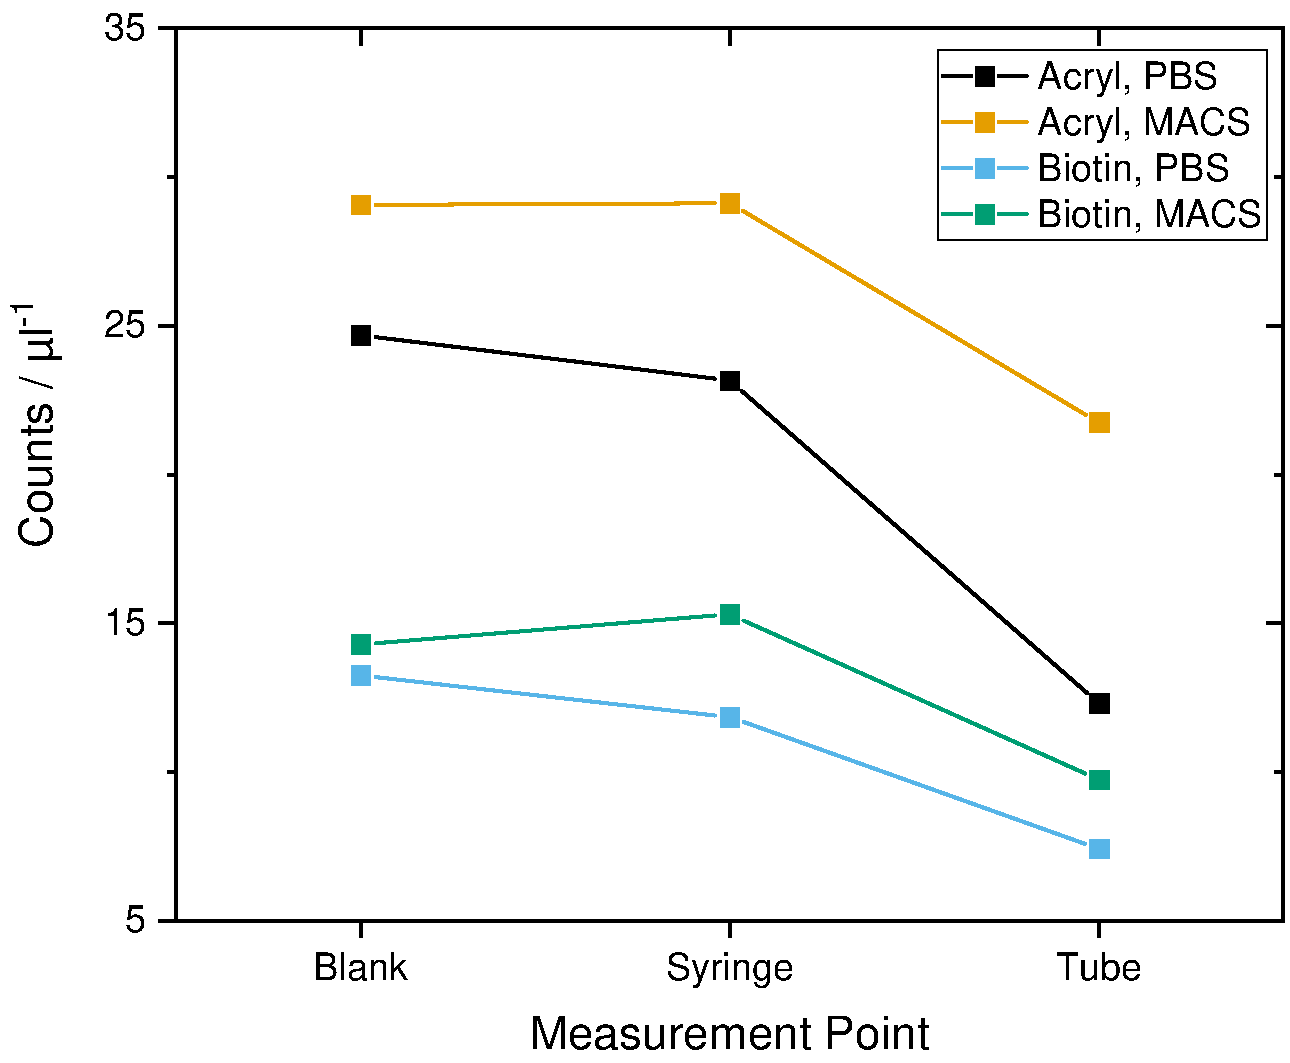
\includegraphics[width=.7\linewidth]{Ressources/Concentration/Losses-Syringe-Tubing}
	\capption{Bead Loss Evaluation in Connectors}{Losses in different buffers and bead surfaces.}
	\label{fig:conc:losses_syringe}
\end{figure}



\subsection{Calibration of Flow Field}
\begin{figure}
	\centering
	\subfloat{
		\subfigimg[height=150pt]{a}{Ressources/Concentration/ConcentrationError}	
	} \hfill
	\subfloat{
		\subfigimg[height=150pt]{b}{Ressources/Concentration/ConcentrationVelocity}	
	}
	\capption{Absolute Concentration Measurements}{Mean from 3 independent measurements(\textbf{a}) mean, sd (\textbf{b}) mean, SEM, Reference Count based error: Liner fit steepness \num{0,34622 +- 0,00968} --> Correction Factor (inverse) \num{2,88833 +- 0,08075}, Velocity Based Correction: $Q/A$ Dims: \SI{700}{\micro\meter}x\SI{50}{\micro\meter} Q = \SI{30}{\micro\liter\per\minute} --> \num{2,26109}}
	\label{fig:conc:AbsConcError}
\end{figure}

\begin{figure}
	\centering
	\subfloat{
		\subfigimg[height=150pt]{a}{Ressources/Concentration/BiotinylWrongCorrection}	
	} \hfill
	\subfloat{
		\subfigimg[height=150pt]{b}{Ressources/Concentration/BiotinylTime}	
	}
	\capption{Error Sources in Concentration Measurements}{(\textbf{a}) mean, SEM Fit factor comparison with protein coated surfaces (\textbf{b}) mean, SEM}
	\label{fig:conc:BiotnylWrongCorr}
\end{figure}

\subsection{Count Stability}
Measurement over 1h

\begin{figure}[!h]
	\centering
	\subfloat{
		\subfigimg[height=150pt]{a}{Ressources/Concentration/BiotinylCountAll}	
	} \hfill
	\subfloat{
		\subfigimg[height=150pt]{b}{Ressources/Concentration/BiotinylTimeAll}	
	}
	\capption{Reproducibility of Concentration Measurements with Saturated Neutravidin Surface}{(\textbf{a}) \SI{80}{\micro\liter\per\minute} mean, SEM (\textbf{b}) All,mean, SEM,}
	\label{fig:conc:All}
\end{figure}



\begin{figure}
	\centering
	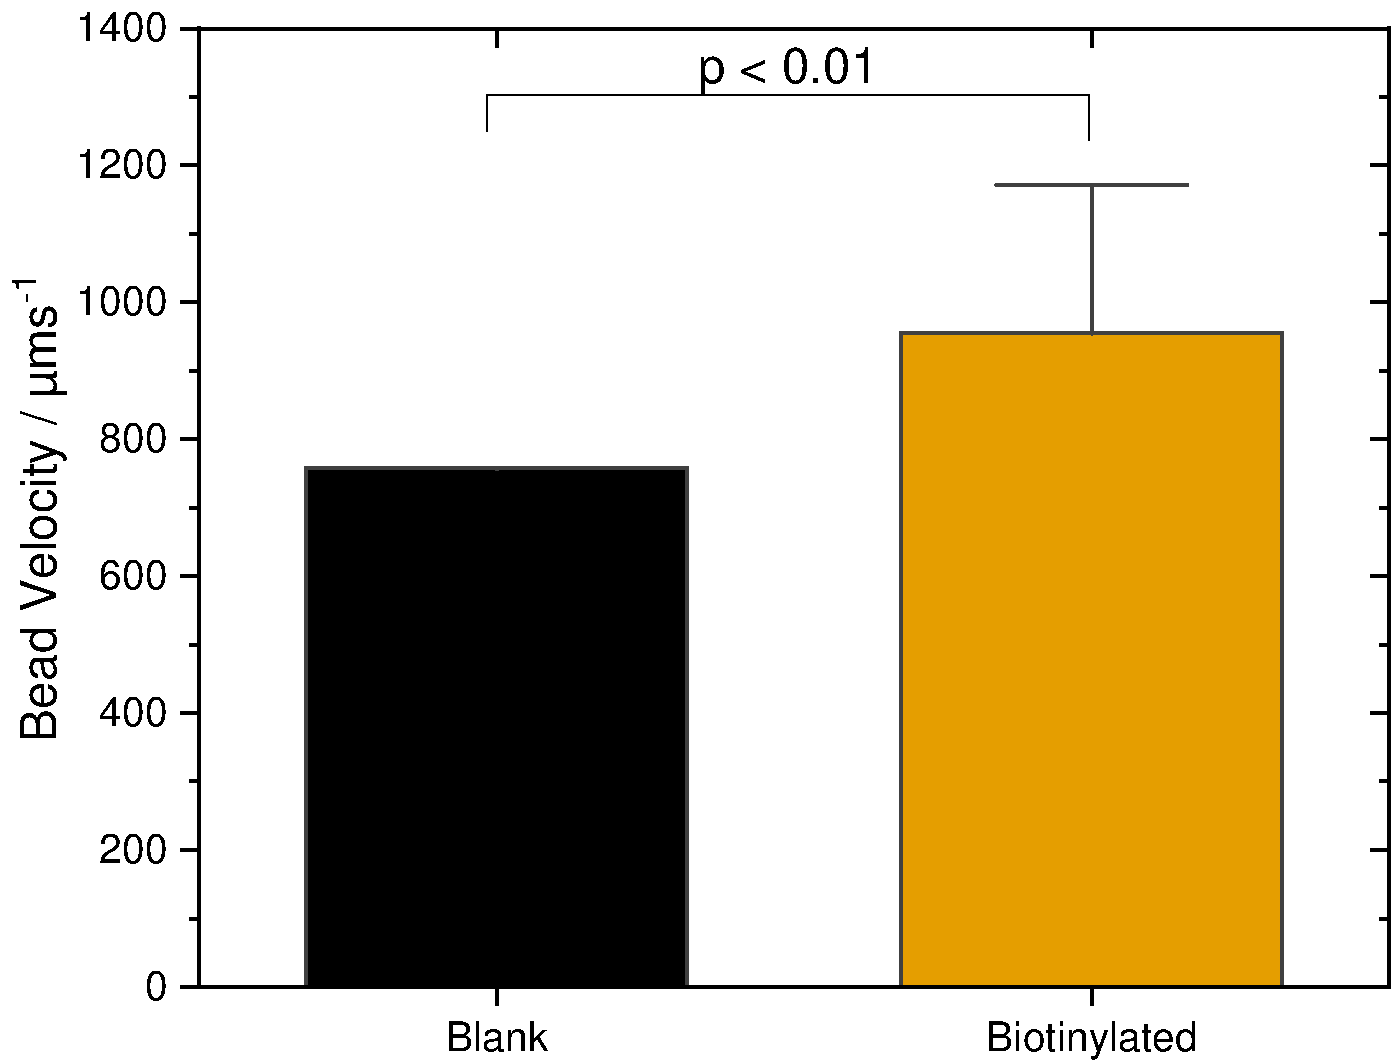
\includegraphics[width=.7\linewidth]{Ressources/Concentration/CaptureVelocity}
	\capption{Measured Bead Velocity}{ p < 0.01}
	\label{fig:conc:vel}
\end{figure}




\subsubsection{Concentration Measurement in Diluted Whole Blood}


\begin{figure}
	\centering
	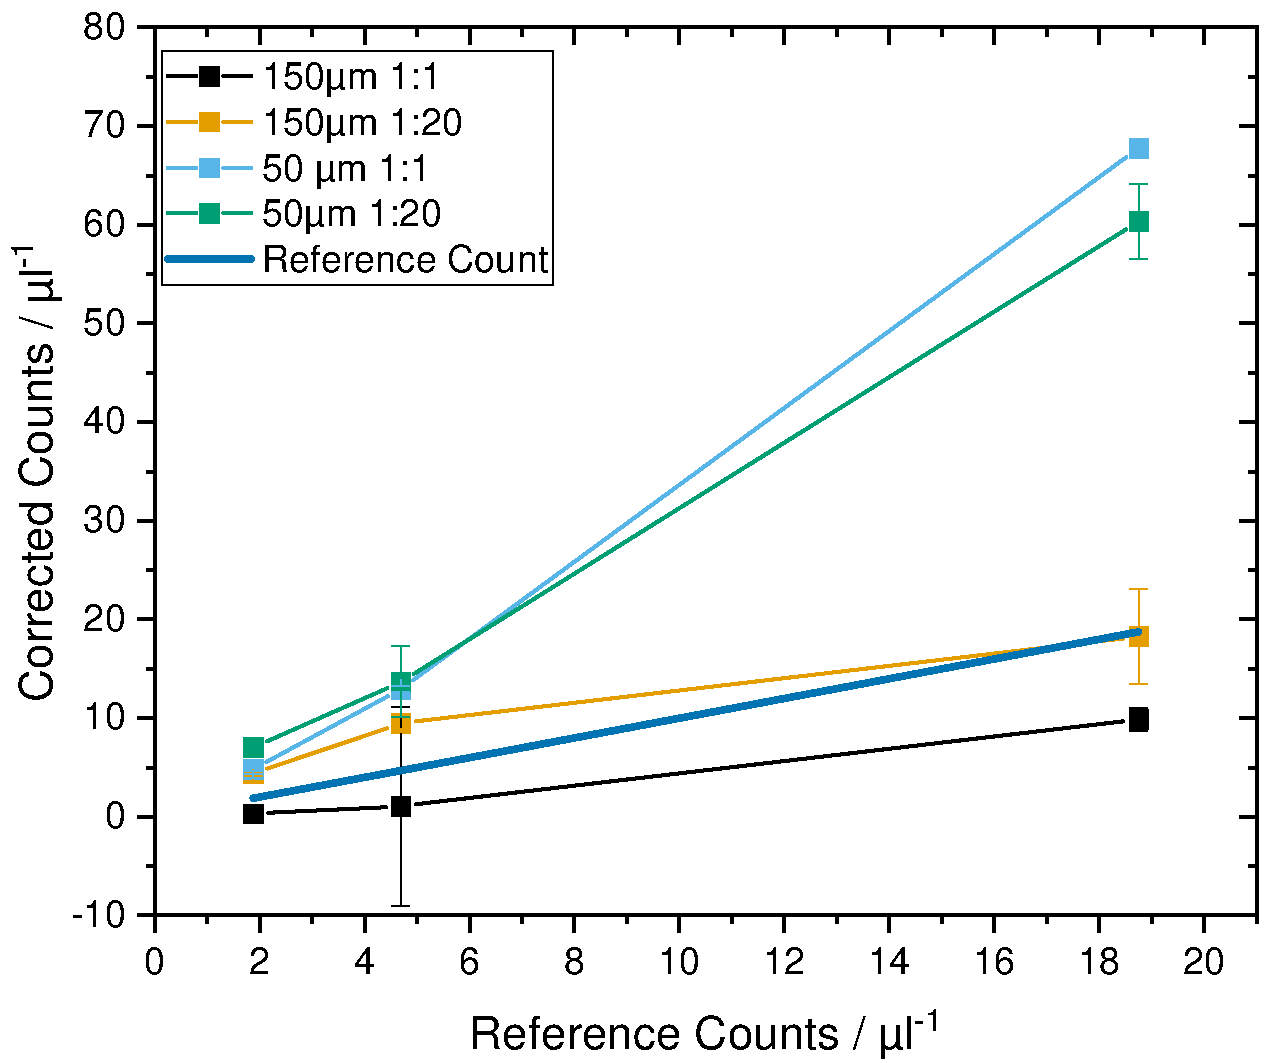
\includegraphics[width=.7\linewidth]{Ressources/Concentration/CorrectionBlood}
	\capption{Absolute Concentration Measurement in Blood Samples Under Varying Channel Height}{Velocity Correction does not work for high concentrations in \SI{50}{\micro\meter}}
	\label{fig:conc:blood}
\end{figure}




\subsection{Differential Counting Setup}

\subsubsection{Sensitivity Calibration}

\begin{figure}
	\centering
	\subfloat{
		\subfigimg[height=150pt]{a}{Ressources/Differential/Optupper}	
	} \hfill
	\subfloat{
		\subfigimg[height=150pt]{b}{Ressources/Differential/Optlower}	
	}
	\capption{Hysteresis Calibration for Stacked \Gls{pcb} }{(\textbf{a}) Optimized for top sensor (\textbf{b}) Optimized for bottom sensor}
	\label{fig:diff:sensitivity}
\end{figure}

\subsubsection{Concentration Measurement in Buffer Solution}



\begin{figure}
	\centering
	\subfloat{
		\subfigimg[height=150pt]{a}{Ressources/Differential/Bottom}	
	} \hfill
	\subfloat{
		\subfigimg[height=150pt]{b}{Ressources/Differential/Top}	
	}
	\capption{Flow Rate Dependency of Counting Setup}{(\textbf{a}) Optimized for top sensor (\textbf{b}) Optimized for bottom sensor}
	\label{fig:diff:flowRate}
\end{figure}

\begin{figure}
	\centering
	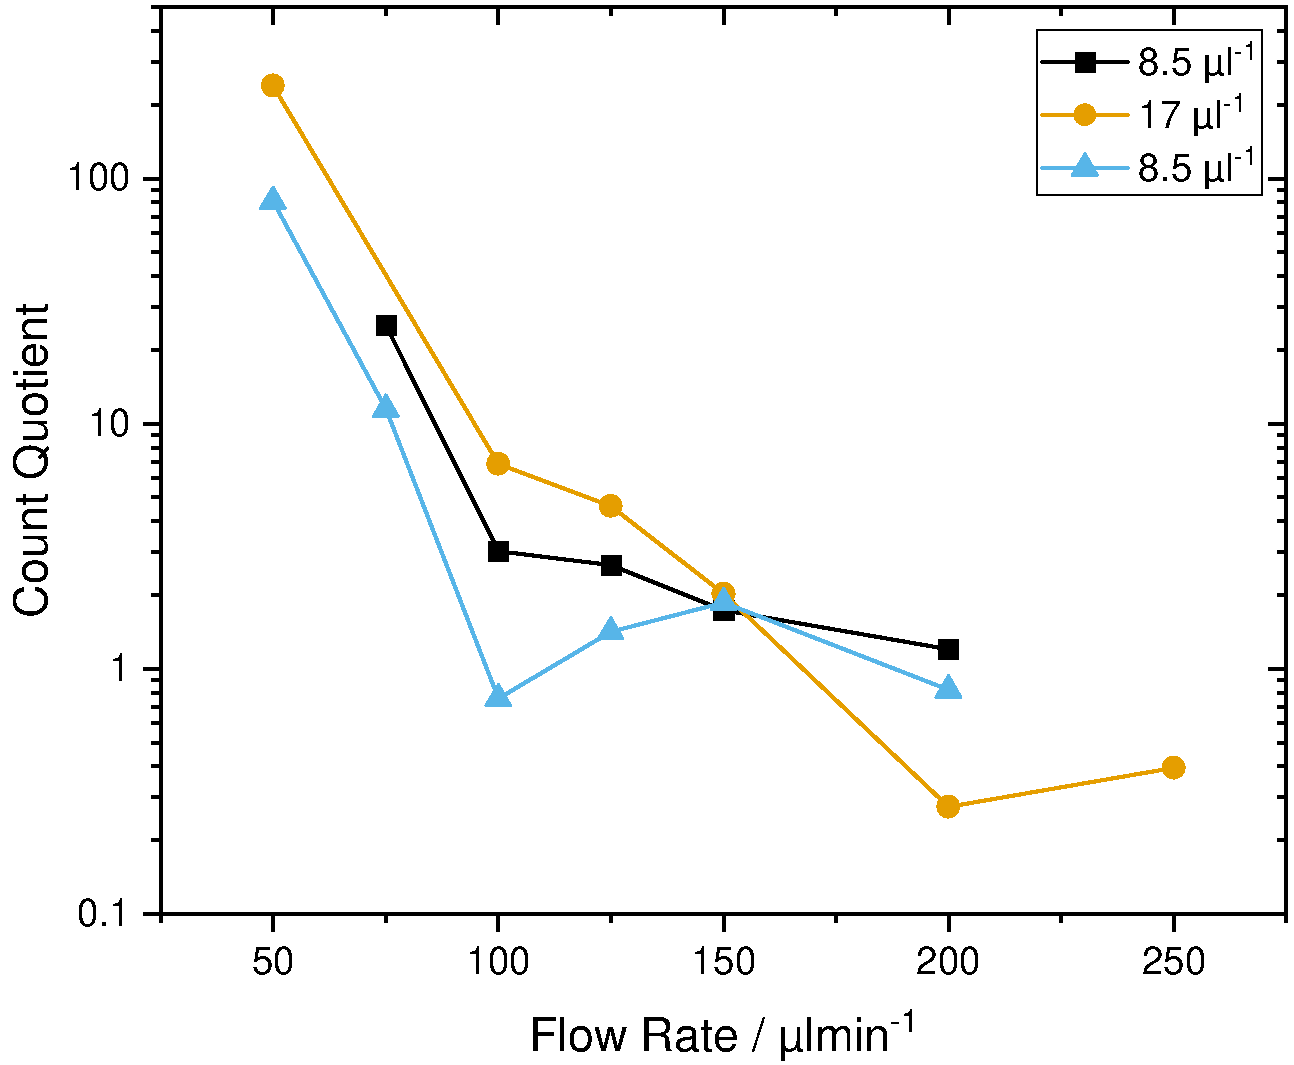
\includegraphics[width=.7\linewidth]{Ressources/Differential/Differential}
	\capption{Optimal Differential Counting Flow Rate}{Losses in different buffers and bead surfaces.}
	\label{fig:conc:optimum}
\end{figure}




\subsection{Surface Magnetization of Biofunctionalized Beads}

Somehow BNF-Dextran showed unspeficity initally, but not anymore later on

\begin{figure}
	\centering
	\subfloat{
		\subfigimg[height=150pt]{a}{Ressources/Concentration/BNFC1}	
	} \hfill
	\subfloat{
		\subfigimg[height=150pt]{b}{Ressources/Concentration/BNFVc}	
	}
	\capption{Bead Coverage Assay with BNF-Dextran-redF-\SI{100}{\nano\meter}}{(\textbf{a}) 1. \SI{80}{\micro\liter\per\minute} 2. \SI{40}{\micro\liter\per\minute} 3. \SI{20}{\micro\liter\per\minute} 4. \SI{10}{\micro\liter\per\minute} (\textbf{b}) d = \SI{8}{\micro\meter}}
	\label{fig:conc:BNF}
\end{figure}



\begin{figure}
\centering
\subfloat{
	\subfigimg[height=150pt]{a}{Ressources/Concentration/OceanC1}	
} \hfill
\subfloat{
	\subfigimg[height=150pt]{b}{Ressources/Concentration/OceanVc}	
}
\capption{Bead Coverage Assay with OceanNanotec \SI{50}{\nano\meter}}{Mean from 3 different particle distributions at maximum coverage, SEM(\textbf{a}) d = \SI{4}{\micro\meter} (\textbf{b}) d = \SI{8}{\micro\meter}}
\label{fig:conc:Ocean}
\end{figure}


\section{Surface Modification and Biofunctionalization of the Sensor Chip Substrate}

\subsection{Physisorption}
Quantification in Plate Reader
Trial with Neutravidin + Sensor (Esthis Versuch)
\clearpage

\begin{figure}
	\centering
	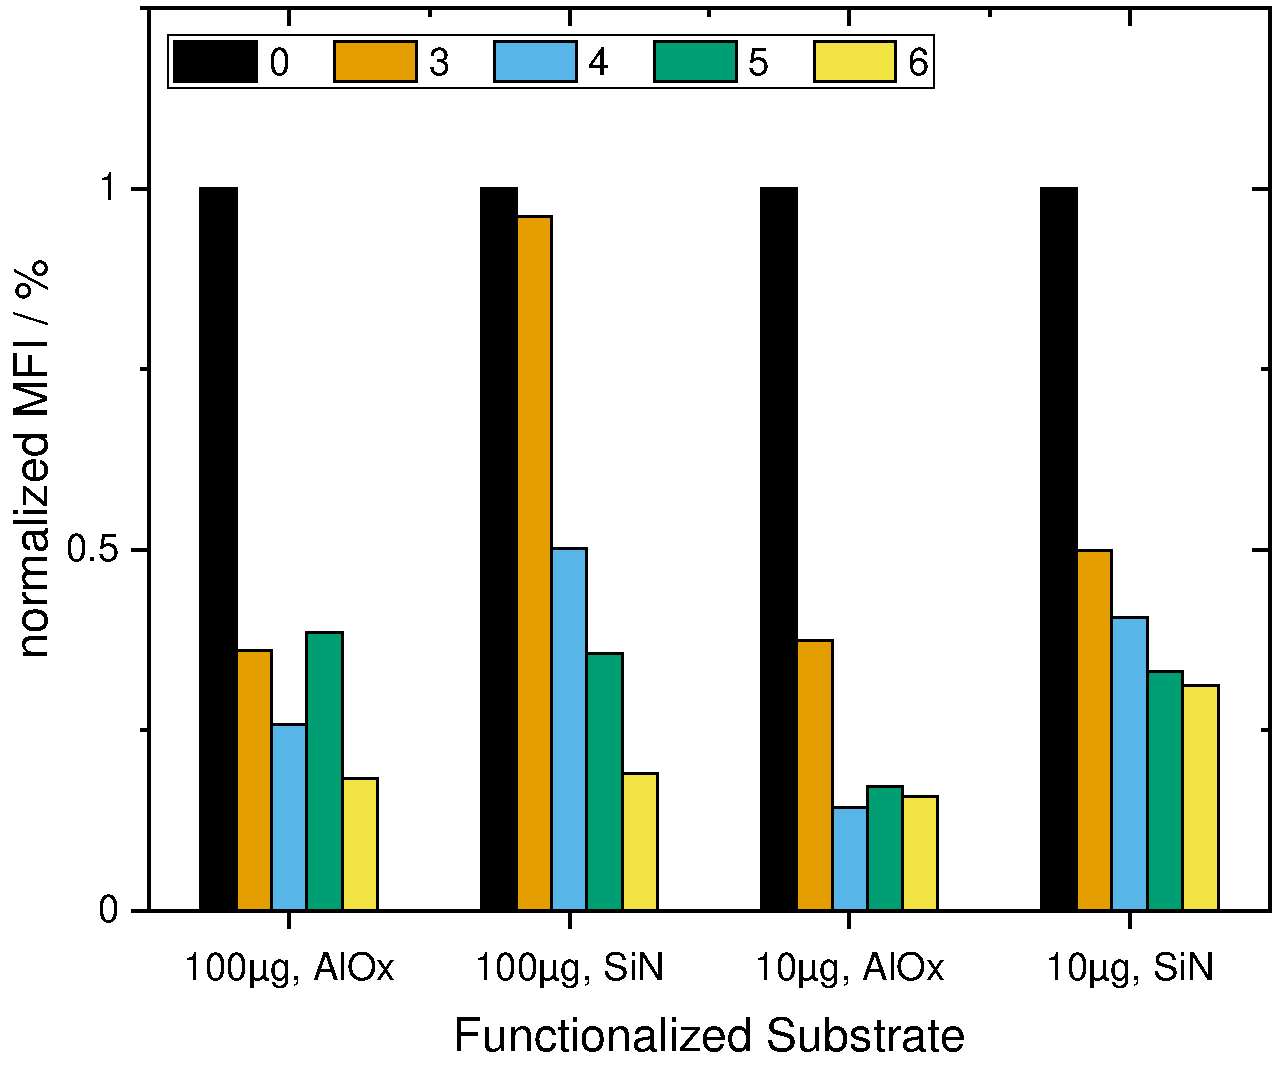
\includegraphics[height=150pt]{Ressources/ResultPlots/SurfaceFuncSiNAlOx}
	\capption{Surface Adsorption Stability of Neutravidin on \Gls{sin} and \Gls{alox}}{Blank with PBS and Blank substrate, corrected, then normalized, absolute protein per \textasciitilde \SI{25}{\milli\meter\square}}
	\label{fig:unsp:wash}
\end{figure}


\subsection{Covalent Attachment}
%\clearpage


\begin{figure}
	\centering
	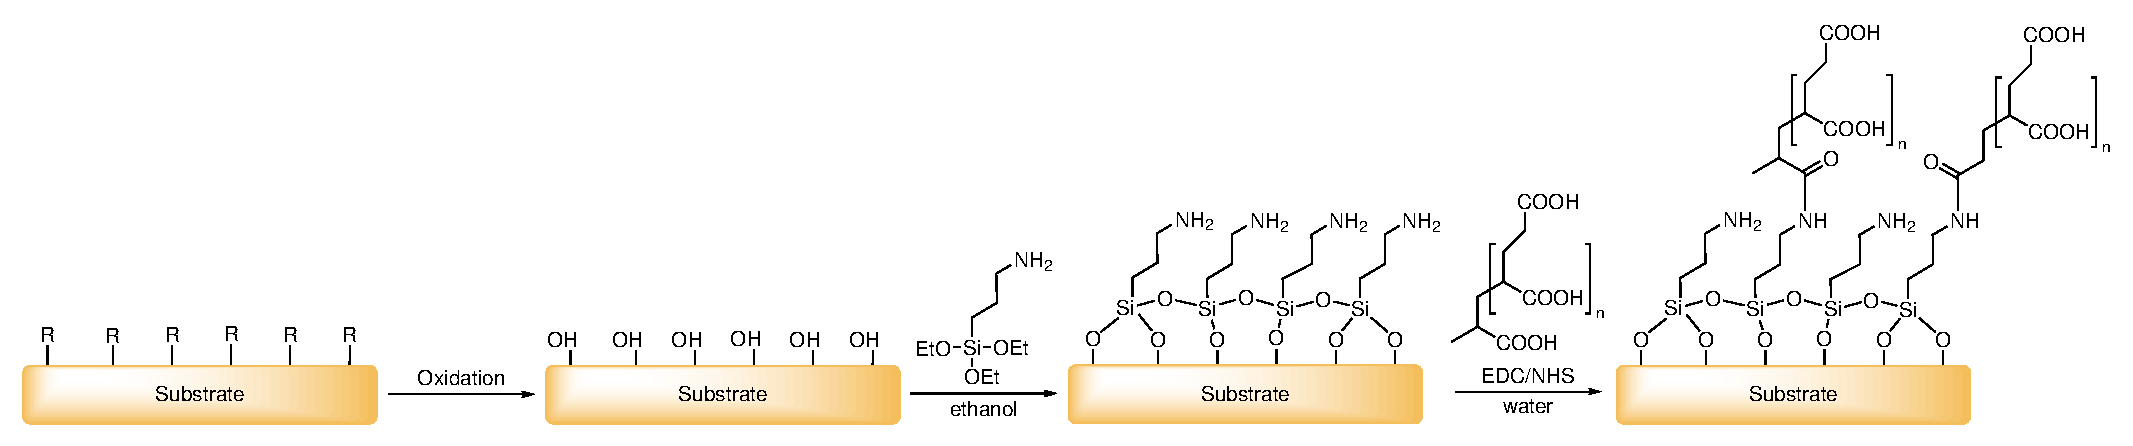
\includegraphics[width=1\linewidth]{Ressources/Chemistry/Substrate}
	\capption{General process chain of chemical surface modification}{Any substrate with various surface groups R (\textbf{a}) is oxidized to exhibit \gls{hydroxyl} groups.(\textbf{b}). Then a silane \gls{sam} is attached (\textbf{c}) and subsequently modified by carbodiimide chemistry with \gls{paa}. (\textbf{d})}
	\label{fig:chem:func:withPAA}
\end{figure}


\begin{figure}
	\centering
	\subfloat{
		\subfigimg[height=150pt]{a}{Ressources/Covalent/SerpentinesDensityCount}	
	} \hfill
	\subfloat{
		\subfigimg[height=150pt]{b}{Ressources/Covalent/NeutravidinTitration}	
	}
	\capption{Neutravidin Titration Fluorescence and Bead Capture Assay}{Relate count to area, then change MFI to counts \si{\per\micro\liter\per\milli\meter\squared}(\textbf{a}) Serpentine (\textbf{b}) Glass}
	\label{fig:coval:fluo}
\end{figure}

\subsubsection{Plasma-Based Approach}
\begin{figure}
	\centering
	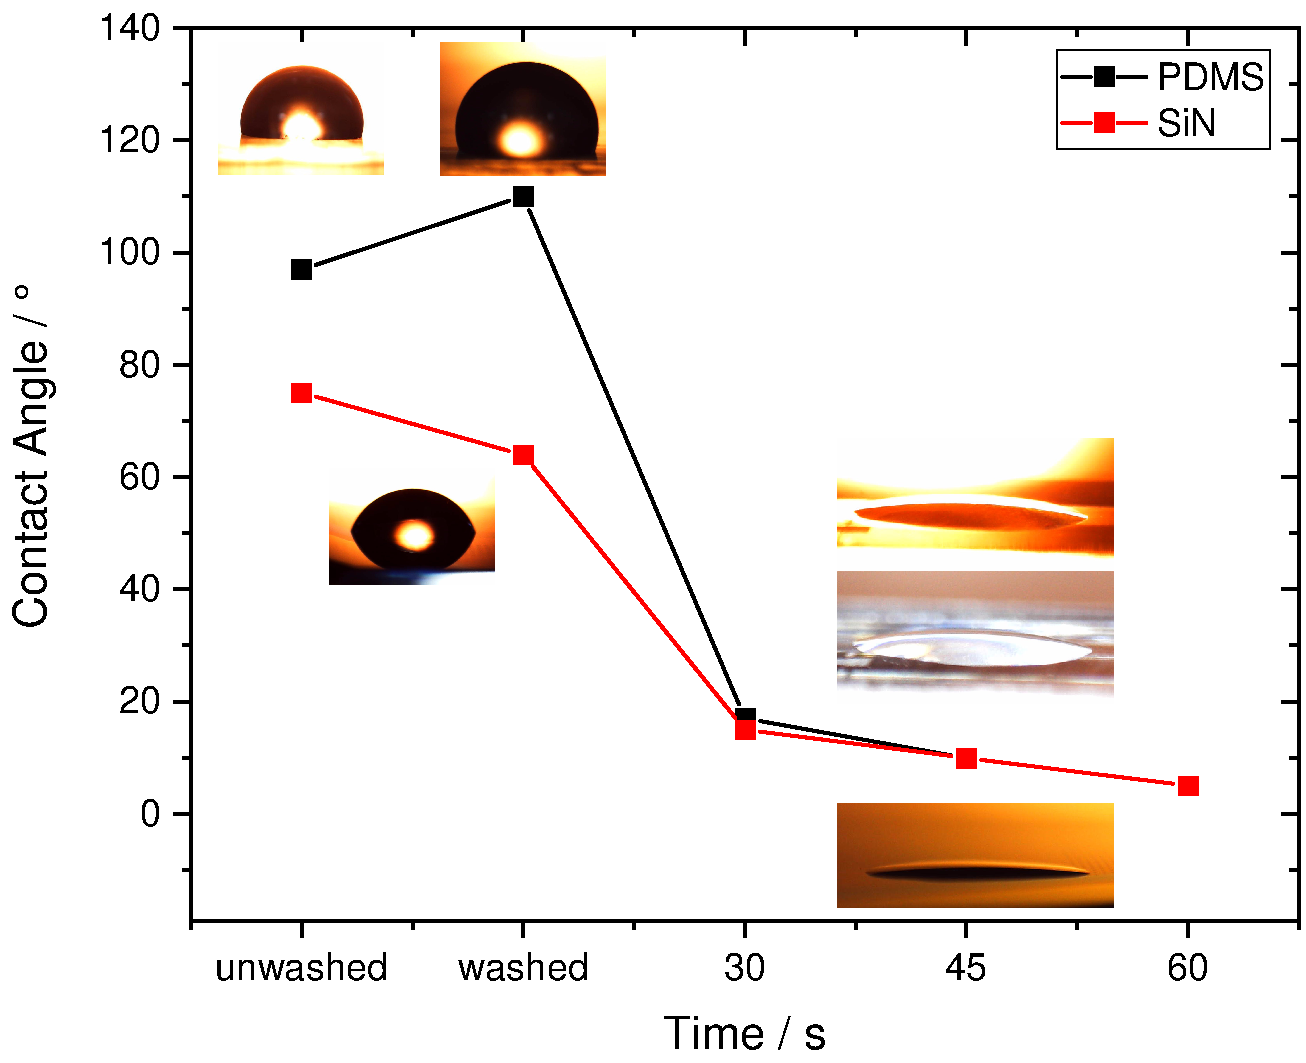
\includegraphics[height=150pt]{Ressources/ResultPlots/PDMS-sessileDrop}
	\capption{Hydrophbicity Analysis of \gls{pdms} under Plasma Exposure}{test123}
	\label{fig:coval:plasma}
\end{figure}


\subsubsection{Water-Based Approach}
Sonicate in Acetone and Water 5'
1:1 \gls{hcl}:Methanol
\gls{h2so4}
Treat for 30 min in light boiling water